\documentclass[12pt]{beamer}
\beamertemplatenavigationsymbolsempty

\usetheme{Copenhagen}
\useoutertheme{infolines}

\usepackage[utf8]{inputenc}
\usepackage[ngerman]{babel}
\usepackage{graphicx}
\usepackage{subfigure}
\title{Task 3 -- Genetische Algorithmen}
\institute{EvoTest}
\author{Alex, Yaroslav, Manuel}
\date{30.11.2016}

\begin{document}
\maketitle 

\section{Letzter Stand}
\begin{frame}{Letzter Stand}
\begin{itemize}
	\item Funktionierende Umwelt
	\begin{itemize}
		\item Logik
		\item Grafische Ausgabe
	\end{itemize}
	\item Größtenteils funktionierender Parkassistent:
	\begin{enumerate}
		\item Berechne den Zielpunkt $\rightarrow$ Funktionierte
		\item Berechne die Fahrspur dorthin $\rightarrow$ Funktionierte sofern das Fahrzeug nicht zu dicht an der Parklücke stand
		\item Berechne aus der Fahrspur die Steuersignale $\rightarrow$ Funktionierte approximativ
		\item Berechne aus den Steuersignalen die Trajektorie (inklusive Distanzberechnung und Kollisionserkennung) $\rightarrow$ Funktionierte
	\end{enumerate}
\end{itemize}
\end{frame}

\section{Bugfixing}
\begin{frame}{Bugfixing}
	\begin{enumerate}
		\item Fahrspurberechnung
		\begin{itemize}
			\item Problem: Geometrische Berechnung suchte iterativ einen bestimmten Punkt auf einer Halbgeraden, die diesen Punkt nicht enthielt
			\item Lösung: Parkvorgang auf diesem Weg nicht möglich $\rightarrow$ Parke nicht direkt ein sondern suche zuerst einen Punkt, von dem aus das einparken geht
		\end{itemize}
		\item Steuersignalberechnung
		\begin{itemize}
			\item Problem: Iterative Berechnung $\rightarrow$ Statt Kreissehne wird eine Tangente gefahren $\rightarrow$ Je größer das Berechnungsintervall, desto größer die Abweichung von der Fahrspur (s. Abbildung \ref{fig:trace})
			\item Lösung: Kreissehne implementiert
		\end{itemize}
	\end{enumerate}
\end{frame}
\begin{frame}
	
	\begin{figure}%
		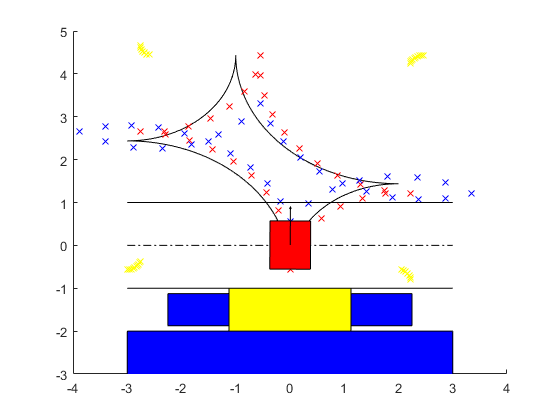
\includegraphics[width=.75\columnwidth]{images/trace}%
		\caption{Fahrspur (schwarz) und tatsächliche Positionen des Fahrzeugs (rot: Hinterachse, blau: Vorderachse)}%
		\label{fig:trace}%
	\end{figure}
\end{frame}

\begin{frame}{Genetische Algorithmen: Implementierung GA}
	\begin{figure}%
	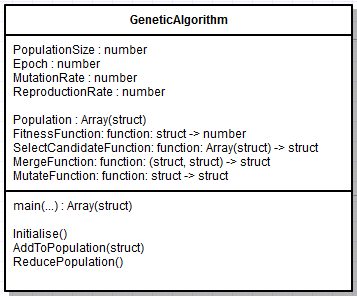
\includegraphics[width=.5\columnwidth]{images/GA_UML}%
	\caption{Klassenkarte Genetischer Algorithmus}%
	\label{fig:GA_CLASS}%
	\end{figure}
\end{frame}

\begin{frame}
	\begin{itemize}
		\item PopulationSize: Größe der Population
		\item Epoch: Akutelle Epoche
		\item MutationRate: Mutations Rate
		\item ReproductionRate: Prozentsatz der Populationsgröße, der zu generieren ist pro Epoche
		\item FitnessFunction: Function-Handle der Fitnessfunktion
		\item SelectCandidateFunction: Function-Handle der Selektionsfunktion
		\item MergeFunction: Function-Handle der Crossover-Funktion
		\item MutateFunction: Function-Handle der Mutationsfunktion
	\end{itemize}
\end{frame}

\begin{frame}{Genetische Algorithmen: Implementierung Chromosom}
	Chromosome enthalten alle Werte, mit denen ein Testszenario eindeutig erzeugt werden kann.
	\begin{itemize}
		\item $\text{Position~}_{\text{Fahrzeug}}$: $(-7.5, -1) \le (X, Y) \le (7.5, 4)~$*
		\item $\text{Orientierung~}_\text{Fahrzeug}$: $0 \le \text{Angle} \le 2 \cdot \pi$
		\item $\text{Größe~}_\text{Parkplatz}$: $(2.25, 1) \le (L, D) \le (5, 2)~$*
	\end{itemize}
	Durch diese Definition ermöglichen wir links und rechts Einpark-Szenarios sowie andere für vorwärts und rückwärts Einparken.\\
	Die Werte werden alle als 8-Bit Integer gespeichert und in die für sie vorgesehene Spanne interpoliert.\\~\\
	\tiny\raggedleft *: elementwise - $\le$
\end{frame}

\begin{frame}{Implementierung: GA-Funktionen}
	\begin{itemize}
		\item Selektion:
		\begin{enumerate}
			\item Standard: $p(\text{chr})=\frac{\text{Fitness}_\text{chr}}{\sum_{c \in \text{Population}} \text{Fitness}_c}$
			\item Alternativ: $p(\text{chr}) = \frac{1}{\text{PopulationSize}}$
		\end{enumerate}
		\item Crossover: Wähle zufällig Werte der "'Eltern"'
		\item Mutation: Jedes Bit wird mit Wahrscheinlichkeit entsprechend der MutationRate geflippt
	\end{itemize}
\end{frame}

\begin{frame}
	\begin{itemize}
		\item Fitness. Kombination durch multiplikation von einzelnen Fitness-Werten:
		\begin{enumerate}
			\item Simpel:\\
			$$\text{Fitness} ~= \frac{1}{1 \,+\, \text{minDistance}}$$
			\item Mindestabstand $dist_{desired}$:\\
			$$\text{Fitness} ~= \frac{dist_{desired}}{\text{minDistance}}$$
			\item Minimaler Parkplatz $(L, D)$:\\
			$$\text{Fitness} ~=\frac{1}{L \,+\, D}$$
			\item Minimaler Abstand zu Simulationsbeginn $dist_{start}$:\\
			$$\text{Fitness} ~= \frac{1}{1 \,+\, dist_{start}}$$
		\end{enumerate}
	\end{itemize}
\end{frame}

\begin{frame}{Probleme}
	\begin{itemize}
		\item Derzeit werden bei PopulationSize = 10 und ReproductionRate = 50\% pro Sekunde nur ungefähr 5 Epochen durchgeführt
		\item Durch den Greedy-Ansatz, der die Population nicht ersetzt, sondern die besten n Chromosome behält, konvergiert der Algorithmus relativ schnell gegen relativ gleiche n Ergebnisse
	\end{itemize}
\end{frame}

\end{document}